\documentclass[14pt]{extarticle}
% math symbols
\usepackage{sfg}


\usepackage{amssymb,amsmath}
\synctex=1
% for different compilers
\usepackage{ifpdf}
% geometry of page
\usepackage[margin=2cm]{geometry}

% if pdflatex, then
\ifpdf
\usepackage[russian]{babel}
\usepackage[utf8]{inputenc}
\usepackage[unicode]{hyperref}
\usepackage[pdftex]{graphicx}
\usepackage{cmlgc}
% if xelatex, then
\else
% math fonts
\usepackage{fouriernc}
% xelatex specific packages
\usepackage[xetex]{hyperref}
\usepackage{xltxtra}	% \XeLaTeX macro
\usepackage{xunicode}	% some extra unicode support
\defaultfontfeatures{Mapping=tex-text}
\usepackage{polyglossia}	% instead of babel in xelatex
\usepackage{indentfirst}	% 
\setdefaultlanguage{russian}
% fonts
\newfontfamily\cyrillicfont{SchoolBookC}
\newfontfamily\cyrillicfontsf{TextBookC}
\setmonofont{Consolas}
\fi

% several pictures in one figure
\usepackage{subfig}
% calc in TeX expressions
\usepackage{calc}
% nice pictures and plots
\usepackage{pgfplots,tikz,circuitikz}
% different libraries for pictures
\usetikzlibrary{%
  arrows,%
  calc,%
  patterns,%
  decorations.pathreplacing,%
  decorations.pathmorphing,%
  decorations.markings,%
  intersections,%
  decorations.text%
}

\usepackage{tkz-euclide}

\usepackage{enumitem}
\renewcommand{\theenumi}{(\asbuk{enumi})}
\renewcommand{\labelenumi}{\asbuk{enumi})}
\AddEnumerateCounter{\Asbuk}{\@Asbuk}{\CYRM}
\AddEnumerateCounter{\asbuk}{\@asbuk}{\cyrm}

\begin{document}

\section*{Задача}

\subsection*{Условие}
Даны две скрещивающиеся прямые $a$ и $b$. Докажите, что существует единственная пара параллельных между собой плоскостей, содержащих эти две прямые.
\subsection*{Решение}
\subsection*{Метод 1}
\subsection*{Доказательство существования.}
Рассмотрим две точки $A\in a$ и $B\in b$. Проведем прямую $b'||b$ через $A$. Аналогично проведем прямую $a'$ через $B$. Получатся две плоскости, содержащие пару параллельных прямых. По второму признаку параллельности, плоскости, содержащие пересекающиеся в одной точке прямые $\alpha=a'b$ и $\beta=ab'$, параллельны. Пример есть.
\subsection*{Доказательство Единственности.}
Докажем от противного. Пусть такая пара плоскостей $\alpha'$ и $\beta'$существует. Заметим, что
\begin{equation}
	A\in\alpha';\, b\subset\beta';\, \alpha||\beta.
\end{equation}
А значит, что $b'\subset \alpha'$. Аналогично $a'\subset\beta'$. Значит, по рассуждению из Доказательства существования, $\alpha'=\alpha$, $\beta'=\beta$.

\newpage

\subsection*{Метод 2}
Пусть $e_0$ -- вектор единичной длины, сонаправленный с $a$. А $e_1$ -- вектор единичной длины, сонаправленный с $b$. Рассмотрим две точки $A\in a$ и $B\in b$. Тогда пусть вектор $e_2=\overrightarrow{AB}/|AB|$. Поскольку прямые $a$ и $b$ скрещивающиеся, Не один из этих векторов не коллинеарен с другим (если $e_0||e_1$, то $a||b$, если $e_0||e_2$, то $B\in a$, аналогично случай $e_1||e_2$). Плоскости $\alpha$ и $\beta$, содержащие прямые $a$ и $b$ параллельны тогда и только тогда, когда $\alpha$ переходит в $\beta$ сдвигом на вектор $\overrightarrow{AB}$. Рассмотрим точку $X\in\alpha$:
\begin{equation}
	X=A + k_0e_0 + k_1e_1 + k_2e_2.
\end{equation}
Теперь посмотрим на точку $Y=X+\overrightarrow{AB}$:
\begin{equation}
	Y=B + k_0e_0 + k_1e_1 + k_2e_2.
\end{equation}
Заметим, что 
\begin{equation}
	BY=k_0e_0 + k_1e_1 + k_2e_2.
\end{equation}
Утверждение ($X\in\alpha\Leftrightarrow Y\in\beta$) равносильно $\alpha||\beta$.

\subsection*{Доказательство существования.}
Плоскости, образуемые векторами $k_2=0, \forall k_0, k_1 \in \mathbb{R}$.
Содержат $a$ при $k_1=0$ и $b$ при $k_0=0$.
\subsection*{Доказательство Единственности.}
Нам точно подходят значения $k_0, k_2=0, \forall k_1 \in \mathbb{R}$, как содержащие $b$ и\newline $k_1, k_2=0, \forall k_0 \in \mathbb{R}$, как содержащие $a$. Также нам подходят их линейные комбинации, как лежащие в той же плоскости. А значит, что пример, приведенный выше, единственный, поскольку плоскость не может содержать в себе другую, отличную от неё плоскость.

\begin{figure}[h]
	\centering
	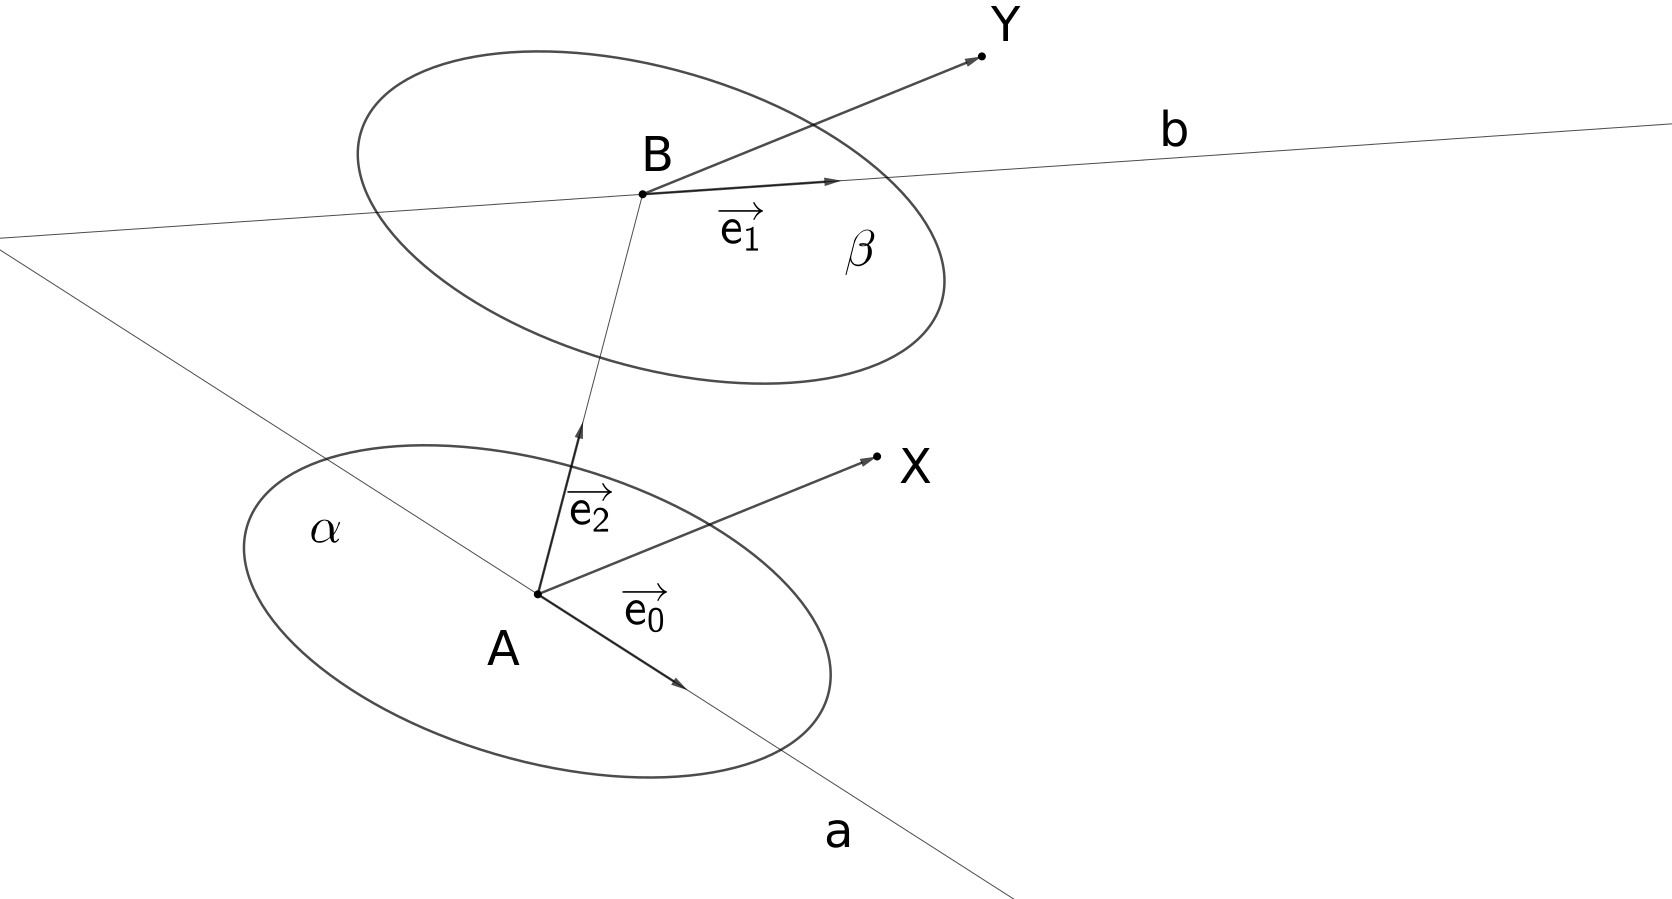
\includegraphics[width=1\textwidth]{{./10.8_1}.png}
\end{figure}
\newpage
\begin{figure}[h]
	\centering
	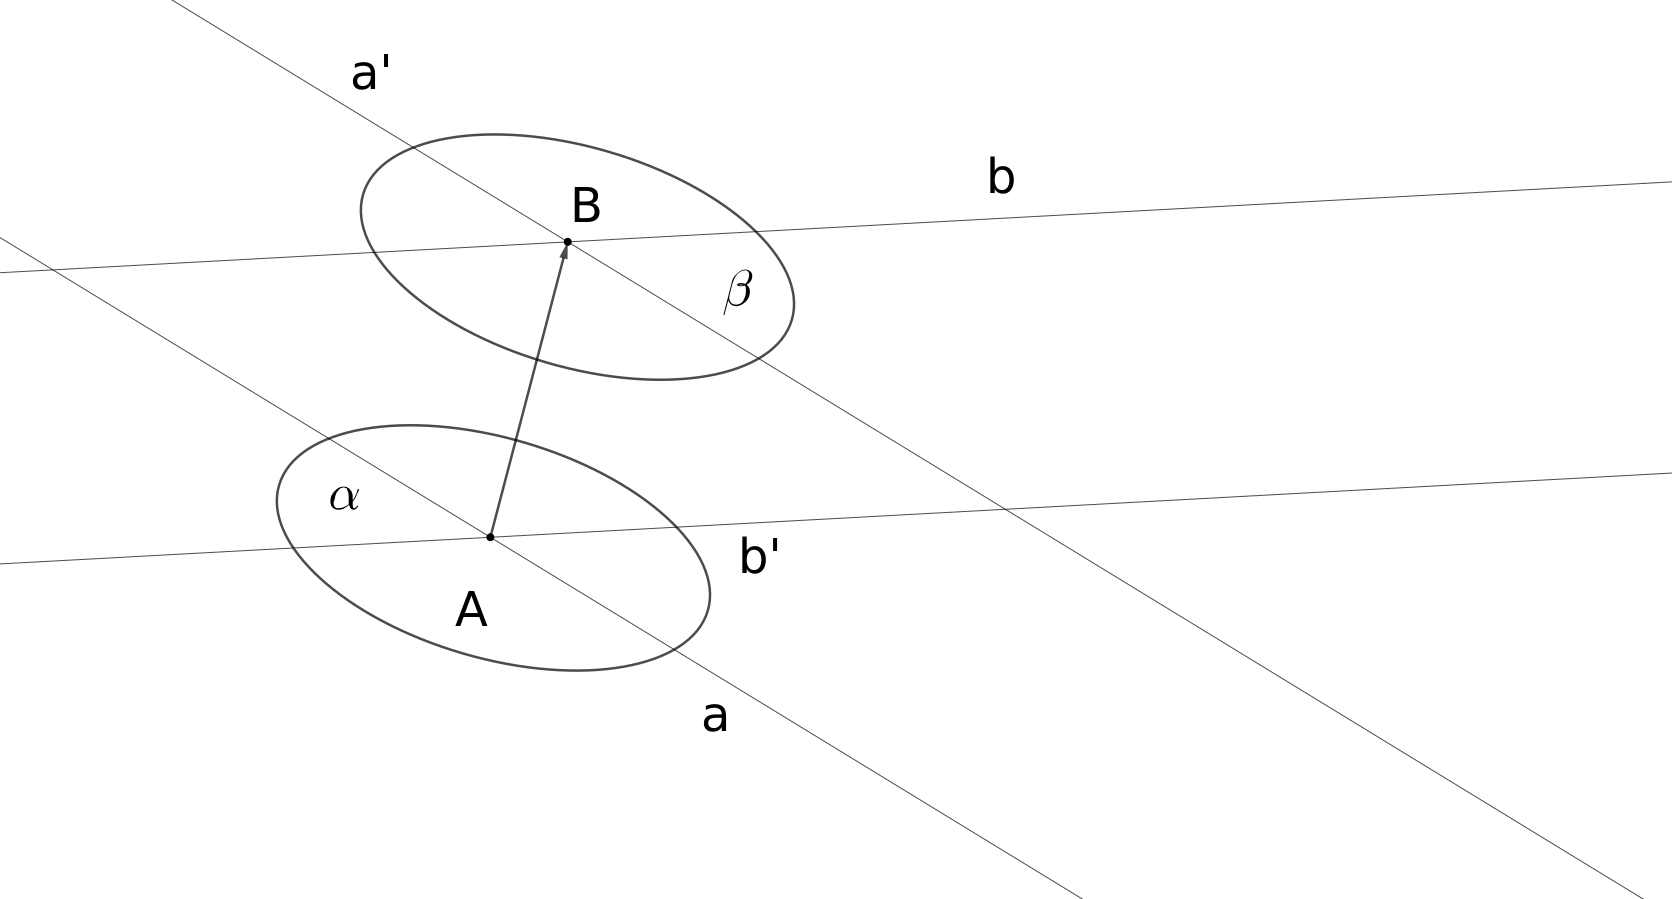
\includegraphics[width=1\textwidth]{{./10.8}.png}
\end{figure}


\end{document}